\documentclass{beamer}
\usetheme{metropolis} 
 
\usepackage[utf8]{inputenc}
\usepackage{amssymb}
\usepackage{amsmath}
\usepackage{amsfonts}
\usepackage{graphicx}
\usepackage{graphics}
\usepackage{setspace}
\usepackage[labelfont=bf]{caption}
\usepackage{sidecap}
\usepackage{placeins}
\usepackage{hyperref}
\usepackage{comment}
\usepackage{fancyhdr} % for the header
\usepackage{lastpage}
\usepackage{indentfirst}
\usepackage{setspace}
\usepackage[space]{grffile}
\usepackage{tabularx}
\usepackage{booktabs}
\usepackage[amssymb]{SIunits}
\usepackage{natbib}
\usepackage{media9}
\usepackage{multicol}

\newcommand{\codeanim}[2]{\uncover<#1->{\texttt{#2}}}
\newcommand{\heapimage}[1]{
\only<#1>{
\includegraphics[width=\textwidth,angle=-90,origin=c]{images/heap/#1}
}
}

%Title Slide% 
\title{CS 6115: Final Project}
\subtitle{Garbage Collection}
\author{Alex Renda (adr74) and Matthew Li (ml927)}
\date{November 29, 2017}
\institute{CS 6115: Certified System Software}

\begin{document}
 
\frame{\titlepage}

\begin{frame}{Overview}

\begin{itemize}
    \item Deep embedding for minimal assembly-like language. Defined small step semantics
    \item Heap is a collection of objects
    \item Shallow embedding for garbage collection.
    \begin{itemize}
        \item Currently mark-sweep
        \item \textit{Hopefully:} mark-sweep-compact
    \end{itemize}
\end{itemize}

\end{frame}

\begin{frame}{Example}
\begin{minipage}{0.45\textwidth}
\codeanim{1}{a := new [ 1 ; 2 ; 3 ]} \\
\codeanim{2}{b := new [ 4 ; 5 ; 6 ]} \\
\codeanim{3}{c := new [ 7 ; 8 ; 9 ]} \\
\codeanim{4}{b := c} \\
\codeanim{5}{a[1] := b} \\
\codeanim{6}{drop a,c} \\
\codeanim{7}{GC} \\
\end{minipage}
\begin{minipage}{0.45\textwidth}
\heapimage{1}
\heapimage{2}
\heapimage{3}
\heapimage{4}
\heapimage{5}
\heapimage{6}
\heapimage{7}
\end{minipage}
\end{frame}


\begin{frame}{Liveness}
\begin{center}
After GC, all objects remaining in the heap are ``reachable'' from at least one of the root variables.

\uncover<2->{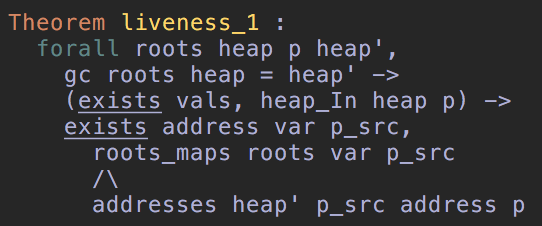
\includegraphics{images/coq/liveness}}

\end{center}
\end{frame}

\begin{frame}{\textit{Hopefully:} Correctness}
All executions  of a program (with GC nondeterministically interleaved) have the same output:

\begin{enumerate}
\item No new crashes are induced
\item GC (including collect) does not change any values that can flow to outputs (e.g. no printing / conditionals on pointer locations)
\end{enumerate}
\end{frame}

\begin{frame}{Safety}
\begin{center}
GC does not remove any objects that are ``reachable'' from a root variable.


\uncover<2->{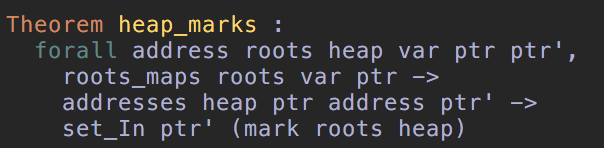
\includegraphics{images/coq/safety}}
\end{center}
\end{frame}

\begin{frame}{(Un)surprisingly Difficult: Representations}

We spent days dealing with artifacts of the representations we chose for our structures:

\begin{itemize}
\item The heap is a graph represented by a list; induction is on addresses
\item List-backed sets required much more manipulation than they should have to get obvious properties (e.g. commutativity)
\end{itemize}

\textbf{Takeaway:} Any nontrivial fact should be an intermediate lemma at the right level of abstraction, structures should be as opaque as possible

\end{frame}
\end{document}